\documentclass[tikz]{standalone}
\usepackage{pgfplots}
\pgfplotsset{compat=1.15}
\usepackage{mathrsfs}
\usetikzlibrary{arrows,calc}
\usepackage{tkz-euclide}
\pagestyle{empty}

\definecolor{AngleClr}{rgb}{0,0.39215686274509803,0}
\definecolor{ShapeClr}{rgb}{0.6,0.2,0}
\definecolor{BlueSqr}{RGB}{5,81,163}

\begin{document}

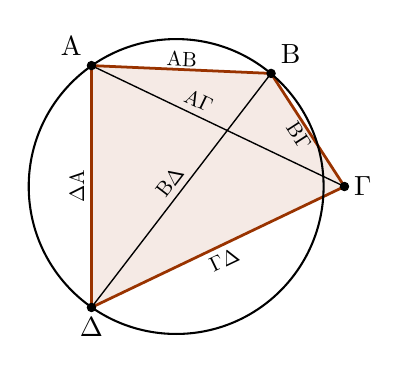
\begin{tikzpicture}[scale=.75]
\tkzSetUpLine[line width=1pt,color=black]
\tkzSetUpPoint[fill=black]

\tkzDefPoint(50:2.5){B}
\tkzDefPoint(125:2.5){A}
\tkzDefPoint(235:2.5){D}
\tkzDefPoint(0:2.85){C}


\tkzDefTriangleCenter[circum](A,B,D) \tkzGetPoint{O}

\tkzFillPolygon[fill=ShapeClr,fill opacity=0.1](A,B,C,D)

\tkzDrawSegments[line width=0.5pt,color=black](A,C B,D)

\tkzDrawPolygon[color=ShapeClr](A,B,C,D)

\tkzDrawCircle[line width=0.75pt,color=black](O,A)


\tkzDrawPoints[size=3](A,B,C,D)

\tkzLabelPoint[above left](A){$\rm A$}
\tkzLabelPoint[above right](B){$\rm B$}
\tkzLabelPoint[right](C){$\rm \Gamma$}
\tkzLabelPoint[below](D){$\rm \Delta$}

\tkzLabelSegments[scale=0.75,above=-0.05cm,sloped](A,B){$\rm AB$}
\tkzLabelSegments[scale=0.75,below=-0.05cm,sloped](B,C){$\rm B\Gamma$}
\tkzLabelSegments[scale=0.75,below,sloped](C,D){$\rm \Gamma\Delta$}
\tkzLabelSegments[scale=0.75,above,sloped](D,A){$\rm \Delta A$}

\tkzLabelSegments[scale=0.75,above,sloped,pos=0.4](A,C){$\rm A\Gamma$}
\tkzLabelSegments[scale=0.75,above,sloped](B,D){$\rm B\Delta$}

\end{tikzpicture}

\end{document}
